\chapter{Application}
\label{chap:application}
The GNN model introduced in \autoref{chap:gnn} will be benchmarked on various datasets in the following sections. All reference data was calculated using the 6-31G(2df,p) basis at theory level B3LYP. 

Models will be evaluated by their iteration count until convergence, by the energy difference from the converged solution the DIIS error (see \autoref{eq:diis_error}), and by the RMSE. The inference time of all models, just a few milliseconds, is roughly three orders of magnitude shorter than that of a typical DFT calculation, and can therefore be regarded as negligible. This performance holds across all applications discussed below.

\section{QM9 - \ch{C7H10O2} Isomers}
\label{sec:qm9_isomers_benchmark}
There are 6095 structural isomers of \ch{C7H10O2} in the QM9 dataset (see \autoref{sec:dataset}). Analogous to the trials performed in \autoref{sec:further_trials_mlp}, we will train and validate on a randomly drawn sample of 500 isomers\footnote{using \textsc{scf\_guess\_datasets} (see \autoref{subsec:gnn_normalization})}. This reduction is necessary to make training and hyperparameter-tuning feasible in the scope of the thesis. Contrary to the full matrix prediction schemes of \autoref{chap:fock_matrix_predictions}, we employ sub-matrix predictions and reconstruct the full matrix, thus increasing the actual number of samples significantly. Per molecule, we obtain 7, 10 and 2 samples for \ch{C}, \ch{H} and \ch{O}, respectively, yielding a total of 3500 \ch{C}, 5000 \ch{H} and 1000 \ch{O} samples. This already provides a certain rotational variability, but additional rotations can be introduced through data augmentation during training to develop a model that is insensitive to rotation when predicting density.
\newpage
\subsection{Initial training}
\label{subsec:qm9_isomers_initial}
%! refer to MGNN_6-31G_NO_AUG_07_07_manual_ref.pth
To evaluate the performance of the GNN devised in \autoref{chap:gnn}, several manual runs were initiated during development, with hyperparameters set to the values listed in \autoref{tab:init_hparams}. 
\begin{table}[H]
    \centering
    \caption[Hyperparameters - initial MGNN training (manually selected)]{Hyperparameters used for the initial MGNN training (manually selected)}
    \label{tab:init_hparams}
    \begin{tabular}{ll ll}
        \toprule
        \textbf{Hyperparameter} & \textbf{Value} & \textbf{Hyperparameter} & \textbf{Value} \\
        \midrule
        Hidden dimension & 256 & Msg. passing rounds & 4 \\
        MsgNet layers & 3 & MsgNet dropout & 15 \% \\
        Batch size & 16 & Grace period & 10 epochs \\
        Target & Density matrix & Loss function & MSE (blockwise) \\
        Learn rate (initial) & $2.68 \times 10^{-3}$ & Weight decay & $1.78 \times 10^{-5}$ \\
        Edge threshold & 3 \AA & Data augmentation & No \\
        \midrule
        Learn rate factor & 0.5 & Learn rate patience & 3 epochs \\
        Learn rate threshold & $10^{-3}$ & Learn rate cooldown & 2 epochs \\
        Learn rate min & $10^{-6}$ & — & — \\
        \bottomrule
    \end{tabular}
\end{table}
Note that these initial runs did not use data augmentation, so the training comprised 400 samples (80\% of our data), leaving 10\% for validation and 10\% for testing. The grace period (time without improvement) was set to 10 epochs to leave the learning rate scheduler sufficient time to take effect.\\

Training and validation losses both monotonically decrease until around epoch 30. As can be seen in \autoref{fig:initial_train_qm9_isomers}, while the loss on the validation set flattens out rather early, training loss decreases throughout the entire training process. 
\begin{figure}[H]
    \centering
    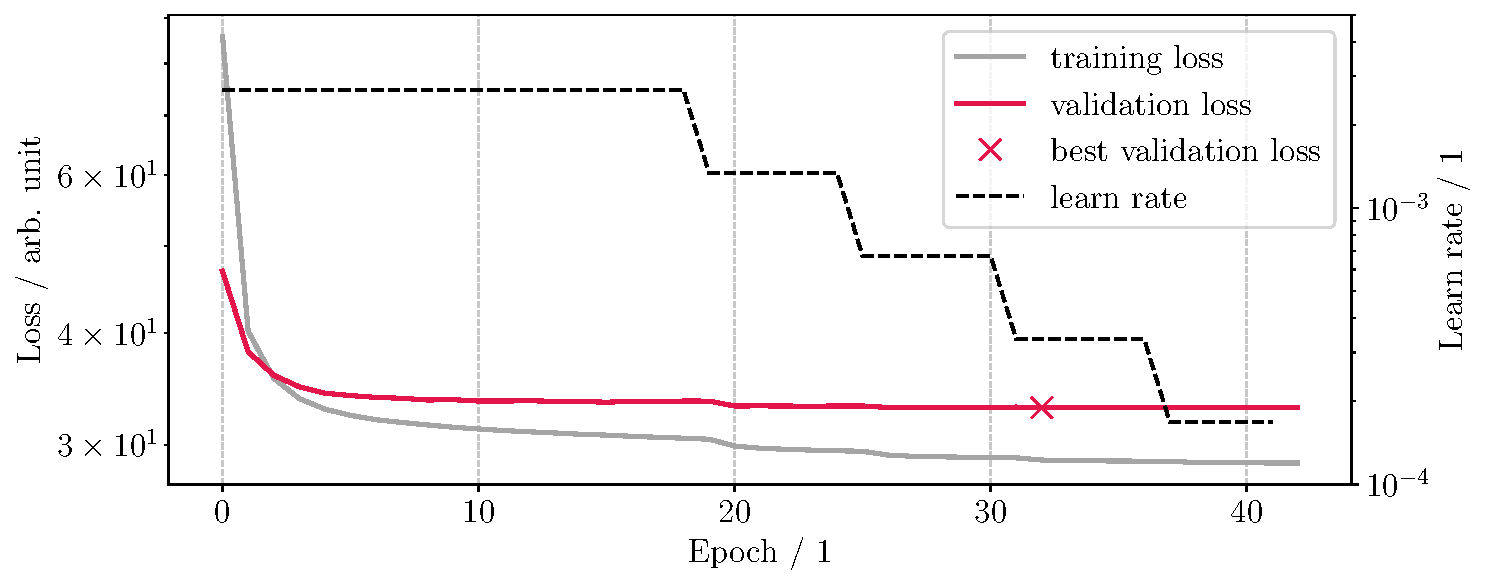
\includegraphics[width=0.8\textwidth]{../fig/gnn/MGNN_6-31G_NO_AUG_07_07_manual_ref_train_val_loss.pdf}
    \caption[Initial GNN loss on QM9-isomers]{Initial GNN training/ validation loss and corresponding learn rate per epoch on QM9-isomers.}
    \label{fig:initial_train_qm9_isomers}
\end{figure}
Both losses are reduced further by stepwise decrease of the learn rate. This run produced the best model in epoch 33, with a validation loss of $33.00$ and a training loss of $28.83$, indicating slight overfitting which is to be expected especially without data augmentation in the training samples. The performance of the model $\text{GNN}_\text{initial}$ on the test set is compared to other models and the various guessing schemes in a summarizing \autoref{tab:qm9_isomers_test_overview} placed at the end of this chapter. 

\subsection{Hyperparameter tuning}
\label{subsec:qm9_isomers_hyperparamtuning}
Validation loss is used as a benchmark to select the best model from a hyperparameter run. While we will also prefer models with lower loss, we must be very careful not to select models which look good on paper but perform worse due to the lack of sufficient correlation between MSE and iteration count. For this reason, we will base our hyperparameter search on the $\text{GNN}_\text{initial}$ model and explore the hyperparameter space in a structured way. 

\textbf{Data augmentation}\\
$\text{GNN}_\text{initial}$ already performed quite well in terms of iterations without using any data augmentation. One might argue that there is already some data augmentation intrinsic to the training set due to the different orientations of atoms in various molecules. 
\begin{figure}[H]
    \centering
    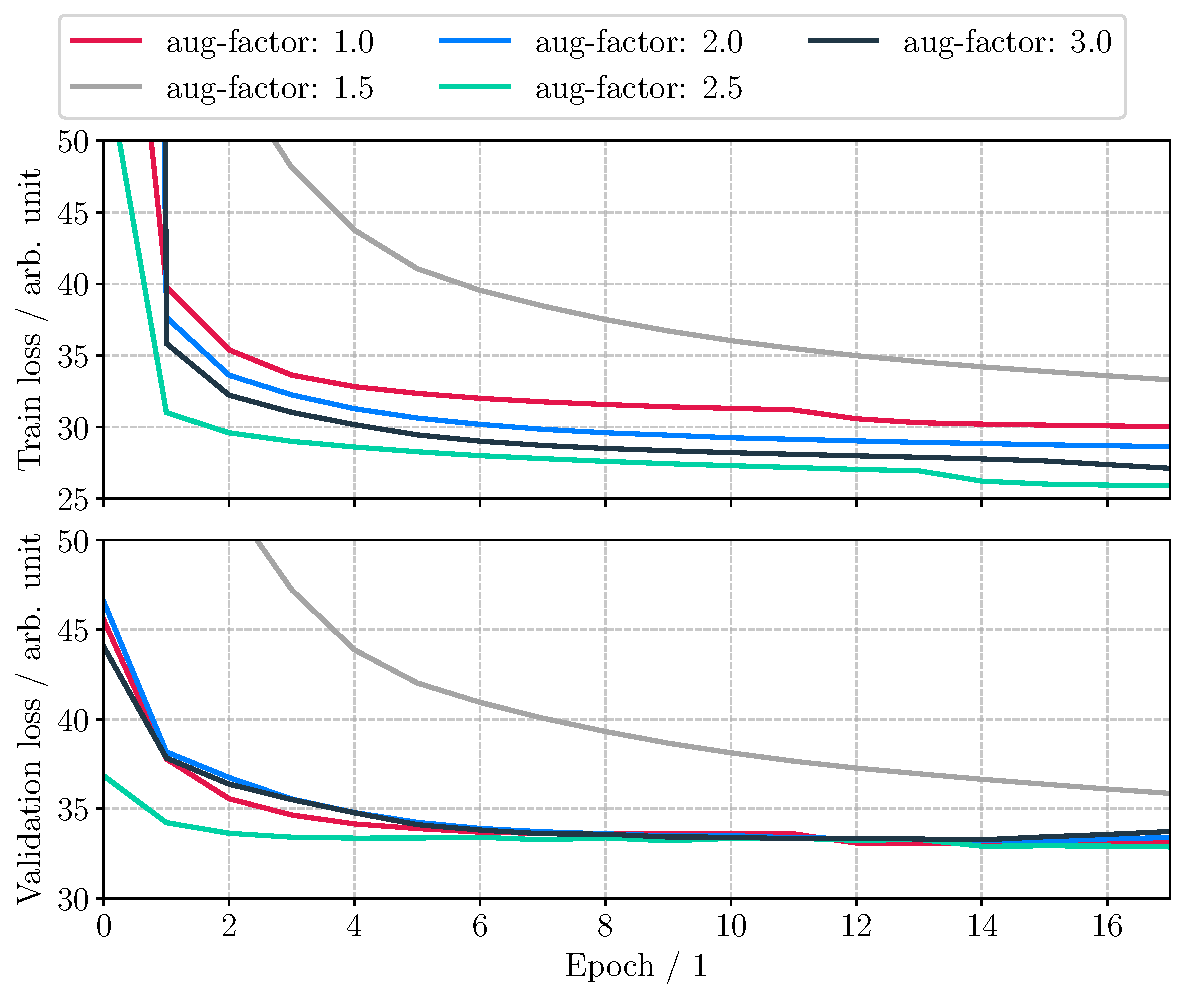
\includegraphics[width=0.75\textwidth]{../fig/application/aug_train_val_loss.pdf}
    \caption[GNN loss for different augmentation factors on QM9-isomers]{GNN loss for different data augmentation factors on QM9-isomers. All other hyperparameters are chosen as in \autoref{tab:init_hparams}.}
    \label{fig:loss_hyper_qm9_isomers}
\end{figure}
A comparison of the training and validation loss between different augmentation factors in \autoref{fig:loss_hyper_qm9_isomers} shows no clear trend regarding the choice of the augmentation factor. While a factor of $2.5$ initially outperforms no augmentation and other factors, they all converge in validation eventually. 
Investigating different metrics on the test set in \autoref{tab:qm9_isomers_data_aug_hyperparam} does not yield a conclusive insight. Our initial model has the best performance in terms of iterations; however, other models do not fall far behind in this metric. Furthermore, no statistically significant correlation was found between the number of iterations and other metrics, including the energy errors ($|\Delta E_\text{DFT}|$ and relative $|\delta E_\text{DFT}|$), the DIIS error, and the RMSE.
\begin{table}[H]
    \centering
    \caption[GNN on QM9 isomers with different data augmentation factors]{GNN performance on the QM9 \ch{C7H10O2} isomers test set for different data augmentation factors\footnotemark. For each factor, the table lists the mean and standard deviation of the following metrics: iterations until convergence, $|\Delta E_\text{DFT}|$ (absolute energy difference to the reference DFT calculation), $|\delta E_\text{DFT}|$ (relative energy difference to the reference DFT calculation), DIIS error (as defined in \autoref{eq:diis_error}), and root mean square error (RMSE) between the predicted and converged density matrices. Energies are given in Hartree ($\unit{\hartree}$).}
    \label{tab:qm9_isomers_data_aug_hyperparam}
    \resizebox{\textwidth}{!}{
        \begin{tabular}{S[table-format=1.1]
                        S[table-format=2.1(1.1)]
                        S[table-format=-1.1(1.1)]
                        S[table-format=-1.4(1.1)]
                        S[table-format=1.3(1)]
                        S[table-format=1.4(1)]}
            \toprule
            {Augmentation factor / 1} & {Iterations / 1} & {$|\Delta E_\text{DFT}|$ / $\unit{\hartree}$}  & {$|\delta E_\text{DFT}|$ / 1} & {DIIS error / $\unit{\hartree}$} & {RMSE / 1} \\
            \midrule
            1.0 & \B 11.2(6)  & \B 0(3) & \B 0.0000(16)  & 0.027(0.004) & \B 0.0078(6) \\
            1.5 & 11.3(6)           & 1.4(17) & 0.0008(10)          & 0.027(0.004) & 0.0079(6)\\
            2.0 & 11.5(6)           & \B 0(3) & 0.0001(14)     & \B 0.027(3)  & 0.0079(6)\\
            2.5 & 12.0(7)           & 1(4)   & 0.001(2)            & 0.029(0.003) & 0.0080(6)\\
            3.0 & 11.4(8)           & 1(3)   & 0.0006(18)          & 0.031(0.007) & 0.0081(6)\\
            3.5 & 11.3(6)           & 2(3)   & 0.0013(18)          & 0.029(0.003) & 0.0080(6)\\
            4.0 & 11.6(10)          & 2(4)    & 0.001(3)            & 0.029(0.003) & 0.0080(6)\\
            \bottomrule
        \end{tabular}
        }
\end{table}
\footnotetext{Other hyperparameters are set according to \autoref{tab:init_hparams}.}
\textbf{Investigating Edge Threshold Distance}\\
The edge threshold distance has an immediate impact on message passing between nodes. It essentially acts as a cutoff that determines whether an edge between two nodes is formed. Keeping it rather short, in the vicinity of bond-lengths will only connect directly bound neighbours. On the other hand, a higher threshold distance allows the formation of longer ranging connections in the GNN. \autoref{tab:qm9_isomers_dist_hyperparam} shows the influence on the metrics for varying threshold distances.  
\begin{table}[H]
    \centering
    \caption[GNN on QM9 isomers with different edge threshold distances]{GNN performance on QM9 \ch{C7H10O2} isomers test set for different edge threshold distances (given in $\unit{\angstrom}$). Other hyperparameters are set according to \autoref{tab:init_hparams}.}
    \label{tab:qm9_isomers_dist_hyperparam}
    \resizebox{\textwidth}{!}{
        \begin{tabular}{S[table-format=1.1]
                        S[table-format=2.1(1.1)]
                        S[table-format=-4(2)]
                        S[table-format=-1.3(2)]
                        S[table-format=1.3(1.1)]
                        S[table-format=1.4(1)]}
                        \toprule
                        {Threshold distance / $\unit{\angstrom}$} & {Iterations / 1} & {$|\Delta E_\text{DFT}|$ / $\unit{\hartree}$}  & {$|\delta E_\text{DFT}|$ / 1} & {DIIS error / $\unit{\hartree}$} & {RMSE / 1} \\
                        \midrule
                        1.5 & 15.1(19)& 1(13)        & 0.001(0.008)   & 0.045(0.005) & 0.0104(5)\\
                        2.0 & 12.3(9) & 4.1(0.8)     & 0.0024(0.0005) & 0.034(0.005) & 0.0084(5)\\
                        2.5 & \B 11.2(6) & 1(2)& 0.0006(0.0012) & 0.026(0.004) & 0.0081(6)\\
                        3.0 & 11.8(13)& 1(6)         & 0.001(0.003)   & 0.027(0.003) & 0.0079(6)\\
                        3.5 & 12.6(8) & 1(2)         & 0.0010(0.0011) & \B 0.025(4) & 0.0077(6)\\
                        4.0 & 12.0(9) & 2(4)         & 0.001(0.002)   & \B 0.025(4) & 0.0078(6)\\
                        4.5 & 12.4(10)& \B 0(7)& \B 0.000(4)& 0.027(0.004) & 0.0080(6)\\
                        5.0 & 11.2(7) & 1(2)         & 0.0005(0.0012) & \B 0.025(4) & \B 0.0077(7)\\
            \bottomrule
        \end{tabular}
    }
\end{table}
For a low distance threshold of $\SI{1.5}{\angstrom}$, which lies around the bond length of \ch{C}-\ch{C} bonds, worse performance in terms of iterations is attained compared to higher threshold distances. 

\textbf{Further hyperparameter optimization runs}\\
For all training runs up until now, the training loss was evaluated only on the normalized sub matrices included in training. In practice, this means that the network has generally lower loss for low cutoff distances because fewer interaction blocks are included in the loss calculation. In the next step, we investigate whether changing the loss to a full matrix loss will impact GNN prediction performance. \autoref{tab:qm9_isomers_further_runs} shows ten different configurations evaluated on the test set. 
\begin{table}[H]
    \centering
    \caption[GNN on QM9 isomers training with full matrix loss]{GNN on QM9 isomers using full matrix loss and a maximum of 30 epochs to train. Metrics on test set and corresponding hyperparameter settings for the five best performing networks (0-4) from search and five sampled ones (5-9) from same hyperparameter search.}
    \label{tab:qm9_isomers_further_runs}
    \resizebox{\textwidth}{!}{
        \begin{tabular}{l
                        S[table-format=2.1(1.1)]
                        S[table-format=-4(2)]
                        S[table-format=-1.3(2)]
                        S[table-format=1.3(1)]
                        S[table-format=1.4(1)]}
            \toprule %!rerun DONE
            Models                 & {Iterations / 1} & {$|\Delta E_\text{DFT}|$ / $\unit{\hartree}$}  & {$|\delta E_\text{DFT}|$ / 1} & {DIIS error / $\unit{\hartree}$} & {RMSE / 1} \\
            \midrule
            $\text{GNN}_\text{f. 0}$ & \B 11.5(9) & 0.7(14)    & 0.0004(8) & 0.028(4) & \B 0.0076(6) \\ %41
            $\text{GNN}_\text{f. 1}$ & 11.6(0.7)        & \B 0.2(17)& \B 0.0001(10)& \B 0.027(4) & 0.0078(0.0006) \\ %73
            $\text{GNN}_\text{f. 2}$ & 11.7(0.8)        & 18.0(18)   & 0.0103(10)& 0.029(3) & 0.0079(0.0006) \\%57
            $\text{GNN}_\text{f. 3}$ & 13.1(1.1)        & 0.3(14)    & 0.0002(8) & 0.035(5) & 0.0084(0.0005) \\ %12
            $\text{GNN}_\text{f. 4}$ & 13.2(1.1)        & 2.3(10)    & 0.0013(6) & 0.040(6) & 0.0088(0.0005) \\ %144
            $\text{GNN}_\text{f. 5}$ & 13.3(1.1)        & 2(3)       & 0.0014(15)& 0.042(4) & 0.0090(0.0005) \\ %95
            $\text{GNN}_\text{f. 6}$ & 13.6(1.0)        & 1(2)       & 0.0004(13)& 0.042(2) & 0.0089(0.0005) \\ %82
            $\text{GNN}_\text{f. 7}$ & 13.9(1.1)        & 1.5(16)    & 0.0008(9) & 0.041(3) & 0.0088(0.0006) \\ %9
            $\text{GNN}_\text{f. 8}$ & 14.5(1.4)        & 0.9(7)     & 0.0005(4) & 0.040(2) & 0.0090(0.0005) \\ %79
            $\text{GNN}_\text{f. 9}$ & 14.7(1.2)        & 7(3)       & 0.0043(18)& 0.042(3) & 0.0091(0.0005) \\ %70
            \bottomrule
        \end{tabular}
    }
        \resizebox{\textwidth}{!}{
        \begin{tabular}{lrrrrrrrrrr}
        \toprule
        Parameters & $\text{GNN}_\text{f. 0}$ & $\text{GNN}_\text{f. 1}$ & $\text{GNN}_\text{f. 2}$ & $\text{GNN}_\text{f. 3}$ & $\text{GNN}_\text{f. 4}$ & $\text{GNN}_\text{f. 5}$ & $\text{GNN}_\text{f. 6}$ & $\text{GNN}_\text{f. 7}$ & $\text{GNN}_\text{f. 8}$ & $\text{GNN}_\text{f. 9}$ \\
        \midrule
        Hidden dimension & 512 & 256 & 128 & 128 & 128 & 512 & 256 & 128 & 256 & 256 \\
        Batch size & 8 & 8 & 8 & 8 & 32 & 32 & 32 & 32 & 32 & 32 \\
        Data aug. factor & 1.83 & 2.46 & 2.38 & 1.76 & 1.50 & 1.14 & 1.67 & 2.45 & 1.91 & 2.33 \\
        Edge threshold & 2.73 & 3.87 & 3.21 & 2.07 & 2.11 & 2.11 & 2.14 & 2.12 & 2.11 & 2.05 \\
        Message passing steps & 2 & 4 & 3 & 3 & 4 & 2 & 3 & 2 & 3 & 3 \\
        Message Net dropout & 0.10 & 0.27 & 0.21 & 0.18 & 0.29 & 0.14 & 0.18 & 0.23 & 0.22 & 0.11 \\
        Message Net layers & 3 & 5 & 4 & 3 & 5 & 3 & 3 & 3 & 5 & 3 \\
        Learn rate & 6.34e-04 & 2.31e-04 & 2.89e-04 & 4.93e-03 & 3.97e-03 & 1.79e-04 & 3.54e-04 & 4.36e-03 & 2.61e-04 & 1.16e-04 \\
        Weight decay & 4.56e-04 & 7.37e-05 & 4.37e-05 & 1.69e-05 & 9.97e-04 & 8.35e-05 & 5.21e-05 & 4.43e-05 & 2.97e-04 & 2.35e-05 \\
        \bottomrule
        \end{tabular}
        }
\end{table}
The best performing networks using full matrix loss perform slightly worse with regard to iteration count. Notably, $\text{GNN}_\text{f. 0}$ reaches the lowest RMSE of all benchmarked models so far. Correlation between our surrogate metrics and iterations is rather high for DIIS and RMSE, with a Pearson correlation coefficient of $0.91$ and $0.94$ respectively. 
Contrary, there is no correlation between the energy errors $|\Delta E_\text{DFT}|$ and $|\delta E_\text{DFT}|$ and the number of iterations. When interpreting these correlations, caution is necessary because they only hold under the specific conditions (GNN trained using full matrix loss) in which they were measured. Below, we will see that these relationships exhibit limited generalizability across different guessing schemes.
\newpage
\subsection{Evaluation \& Conclusion}
\label{subsec:qm9_isomers_eval_and_concl}
The top performing models as defined above are now compared to \textsc{PySCF} guessing schemes. A summary of this comparison is provided in \autoref{tab:qm9_isomers_test_overview}.
\begin{table}[H]
    \centering
    \caption[Models compared to \textsc{PySCF} and $\overline{P}$ schemes - \ch{C7H10O2} Isomers]{Comparison of different models with \textsc{PySCF} and $\overline{P}$ guessing schemes for QM9 - \ch{C7H10O2} Isomers.}
    \label{tab:qm9_isomers_test_overview}
    \resizebox{\textwidth}{!}{
        \begin{tabular}{l
                        S[table-format=2.1(1.1)]
                        S[table-format=-4(3)]
                        S[table-format=-1.3(2)]
                        S[table-format=1.4(1.1)]
                        S[table-format=1.4(1)]}
            \toprule
            Guessing schemes                 & {Iterations / 1} & {$|\Delta E_\text{DFT}|$ / $\unit{\hartree}$}  & {$|\delta E_\text{DFT}|$ / 1} & {DIIS error / $\unit{\hartree}$} & {RMSE / 1} \\
            \midrule
            $\text{GNN}_\text{initial}$   &11.2(6)   & \B 0(3)& \B 0.0000(16) & 0.027(0.004) & 0.0078(6)\\ %initial
            $\text{GNN}_\text{f. 0}$      & 11.5(9)  & 0.7(14)    & 0.0004(8) & 0.028(4) & \B 0.0076(6) \\ %41
            $\overline{P}$                & 17.1(15) & 211(6)      & 0.1208(19)& 0.110(3)  & 0.0137(4)\\
            \texttt{1-e}                  & 18.8(18) & 220(30)     & 0.128(19) & 0.1220(10)& 0.14(4)  \\
            \texttt{vsap}                 & 14.2(9)  & 5.4(4)      & 0.0030(2) & \B 0.026(2) & 0.0109(7)\\
            \texttt{atom}                 & 16.6(19) & 14(4)       & 0.007(3)  & 0.044(7) & 0.016(2) \\
            \texttt{minao}                & \B 10.8(6)& 2.8(2)&0.00162(12)& 0.077(3) & 0.0155(4)\\
            \bottomrule
        \end{tabular}
    }
\end{table}
A direct comparison of \textsc{PySCF} and $\overline{P}$ guessing schemes with our GNN approach already offers several insights. Examining the relationship between energy errors and the number of iterations shows that guesses with smaller energy errors ($|\Delta E_\text{DFT}|$) tend to convergence faster. 
Furthermore, a low DIIS alone will not necessarily translate into fast convergence of the guessed density. The GNN approach surpasses most conventional guessing schemes and performs nearly on par with \texttt{minao} in terms of iterations. Varying the data augmentation factor had negligible effect on the convergence speed, while the distance threshold contributes for distances around the bond length. However, it remains to be seen how well these models generalize to other data. 

\section{QM9 - \ch{C7H10O2} Molecular Dynamics (MD)}
\label{sec:qm9_md_isomers_benchmark}
So far, all predictions have considered only ground state geometries. While predicted and calculated traits of the ground state give invaluable insight into the chemical properties, the behaviour of the molecules in more attainable environments is of interest. The MD trajectories of \ch{C7H10O2} dataset \parencite{ref:qm9_isomers_md} constitute a randomly sampled set of 113 isomers from the QM9 \ch{C7H10O2} data. The trajectory of every isomer is calculated every $\SI{1}{\femto\second}$ for 5000 steps at a temperature of 500 K using the PBE exchange-correlation potential (see \ref{subsec:background_dft}). From these geometries, 500 are sampled to calculate a reference data set using the 6-31G(2df,p) basis at the B3LYP level of theory. This combination is employed in all following computer experiments. 
\newpage
\subsection{Zero-shot predictions}
\label{sec:qm9_md_isomers_zero_shot}
Zero-shot predictions are made on inputs outside the training set's scope. In our case, a model previously trained on the QM9 \ch{C7H10O2} isomer set may be used to predict the density for a given MD sample. Prediction metrics using the pre-trained models from \autoref{sec:qm9_isomers_benchmark} on the MD test set are given in \autoref{tab:qm9_md_zero_shot}. 
\begin{table}[H]
    \centering
    \caption[GNN zero-shot predictions on QM9 \ch{C7H10O2} isomer MD]{GNN zero-shot predictions on the QM9 \ch{C7H10O2} isomer MD test set. $\text{GNN}_\text{initial}$ and $\text{GNN}_\text{f. 0}$ were trained using the QM9 \ch{C7H10O2} isomer set.}
    \label{tab:qm9_md_zero_shot}
    % \resizebox{\textwidth}{!}{
        \begin{tabular}{l
                        S[table-format=2.1(1)]
                        S[table-format=-4(2)]
                        S[table-format=-1.3(1.1)]
                        S[table-format=1.2(1.1)]
                        S[table-format=1.4(1.1)]}
            \toprule
            Models                 & {Iterations / 1} & {$|\Delta E_\text{DFT}|$ / $\unit{\hartree}$}  & {$|\delta E_\text{DFT}|$ / 1} & {DIIS error / $\unit{\hartree}$} & {RMSE / 1} \\
            \midrule
            $\text{GNN}_\text{initial}$   & 11.4(9)    & 1(2)     & 0.0007(11)  & 0.026(3)& 0.0079(4) \\ %!- do full rerun + iterations with model from data_aug_1.0 -> done and already updated
            $\text{GNN}_\text{f. 0}$      & 11.3(8)  & 1.3(1.1) & 0.0007(6)     & 0.029(3)& 0.0077(4) \\
            \bottomrule
        \end{tabular}
    % }
\end{table}
Both models perform surprisingly well on the unseen data. $\text{GNN}_\text{f. 0}$ even performs slightly better, indicating a generalization to various perturbations of the geometry. Furthermore, $\text{GNN}_\text{initial}$ performs slightly worse on the MD dataset.

\subsection{Hyperparameter tuning}
\label{sec:qm9_md_isomers_hyp_tuning}
%! full matrix run in tune_logs_MGNN_hyp_small_full_mat_loss_md
Metrics for re-trained versions of $\text{GNN}_\text{initial}$ and $\text{GNN}_\text{f. 0}$ from \autoref{sec:qm9_isomers_benchmark} are shown in \autoref{tab:qm9_md_last_best_retrain}. While training $\text{GNN}_\text{f. 0}$ on the MD dataset leads to improvements in all metrics, the re-trained version of $\text{GNN}_\text{initial}$ performs worse than the original model on the MD test set.  
\begin{table}[H]
    \centering
    \caption[GNN predictions on QM9 \ch{C7H10O2} isomer MD]{GNN predictions on the QM9 \ch{C7H10O2} isomer MD test set. With MD-re-trained\footnote{models marked with a $*$ are architectures from another dataset re-trained on the current one} versions of $\text{GNN}_\text{initial}$ and $\text{GNN}_\text{f. 0}$.}
    \label{tab:qm9_md_last_best_retrain}
    % \resizebox{\textwidth}{!}{
        \begin{tabular}{l
                        S[table-format=2.1(1.1)]
                        S[table-format=-4(2)]
                        S[table-format=-1.3(2)]
                        S[table-format=1.3(2)]
                        S[table-format=1.4(1)]}
            \toprule
            Models                 & {Iterations / 1} & {$|\Delta E_\text{DFT}|$ / $\unit{\hartree}$}  & {$|\delta E_\text{DFT}|$ / 1} & {DIIS error / $\unit{\hartree}$} & {RMSE / 1} \\
            \midrule
            $\text{GNN}^{\text{MD*}}_\text{initial}$   & 12.3(10)  & 1(4) & 0.001(2)      & 0.035(4)& 0.0086(6) \\ %! comp_models initial - rerun! 
            $\text{GNN}^{\text{MD*}}_\text{f. 0}$      & 11.1(5)  & 0.0(1.0) & 0.0000(6)  & 0.028(3)& 0.0073(5) \\ % comp_models f0
            \bottomrule
        \end{tabular}
    % }
\end{table}
Analogous to the hyperparameter optimization in \autoref{tab:qm9_isomers_further_runs}, we also use full matrix loss for hyperparameter tuning of the specialized MD models in \autoref{tab:qm9_md_further_runs}. Comparing \autoref{tab:qm9_isomers_further_runs} and \autoref{tab:qm9_md_further_runs}, heavier regularization is generally observed in the MD models. Higher data augmentation and a slightly stronger weight decay help with fitting the varied density given by the perturbed geometries. Furthermore, four out of the top five networks have a batch size of eight, introducing more noise and thus regularization into the update steps. \\
\begin{table}[H]
    \centering
    \caption[GNN on QM9 isomers MD training with full matrix loss]{GNN on QM9 isomers MD using full matrix loss and a maximum of 30 epochs to train. Metrics on test set and corresponding hyperparameter settings for the ten best performing networks in terms of iterations.}
    \label{tab:qm9_md_further_runs} %!TODO rerun with all models if there is time!
    \resizebox{\textwidth}{!}{
        \begin{tabular}{l
                        S[table-format=2.1(2)]
                        S[table-format=-4(2)]
                        S[table-format=-1.3(2)]
                        S[table-format=1.3(1)]
                        S[table-format=1.4(1)]}
            \toprule
            Models                 & {Iterations / 1} & {$|\Delta E_\text{DFT}|$ / $\unit{\hartree}$}  & {$|\delta E_\text{DFT}|$ / 1} & {DIIS error / $\unit{\hartree}$} & {RMSE / 1} \\
            \midrule
            $\text{GNN}^{\text{MD}}_\text{f. 0}$ & \B 10.9(5) &  1.5(1.7) & 0.001(0.001) & \B 0.027(3) & \B 0.0075(4) \\
            $\text{GNN}^{\text{MD}}_\text{f. 1}$ & 11.0(4) &   1.8(1.3)  & 0.001(0.001) & 0.030(0.003) & 0.0076(0.0004) \\
            $\text{GNN}^{\text{MD}}_\text{f. 2}$ & 11.2(6) &   3.1(2.2)  & 0.002(0.001) & 0.031(0.003) & 0.0079(0.0005) \\
            $\text{GNN}^{\text{MD}}_\text{f. 3}$ & 11.2(4) &   1.9(2.1)  & 0.001(0.001) & 0.033(0.003) & 0.0084(0.0003) \\
            $\text{GNN}^{\text{MD}}_\text{f. 4}$ & 11.4(6) &   3.5(1.2)  & 0.002(0.001)  & 0.031(0.003) & 0.0081(0.0003) \\
            $\text{GNN}^{\text{MD}}_\text{f. 5}$ & 11.6(10)&   0.6(2.3)  & \B 0.000(1)  & 0.035(0.003) & 0.0087(0.0005) \\
            $\text{GNN}^{\text{MD}}_\text{f. 6}$ & 11.6(9) &   \B 0.0(1.8)  & \B 0.000(1)  & 0.035(0.009) & 0.0087(0.0012) \\
            $\text{GNN}^{\text{MD}}_\text{f. 7}$ & 11.8(9) &   1.0(3.3)  & 0.001(0.002)  & 0.032(0.004) & 0.0084(0.0004) \\
            $\text{GNN}^{\text{MD}}_\text{f. 8}$ & 11.8(7) &   4.1(2.0)  & 0.002(0.001) & 0.037(0.003) & 0.0085(0.0003) \\
            $\text{GNN}^{\text{MD}}_\text{f. 9}$ & 11.8(7) &   1.0(1.8)  & 0.001(0.001)  & 0.035(0.006) & 0.0083(0.0009) \\
            \bottomrule
        \end{tabular}
    }
        \resizebox{\textwidth}{!}{
        \begin{tabular}{lrrrrrrrrrr}
        \toprule
        Parameters & $\text{GNN}^{\text{MD}}_\text{f. 0}$ & $\text{GNN}^{\text{MD}}_\text{f. 1}$ & $\text{GNN}^{\text{MD}}_\text{f. 2}$ & $\text{GNN}^{\text{MD}}_\text{f. 3}$ & $\text{GNN}^{\text{MD}}_\text{f. 4}$ & $\text{GNN}^{\text{MD}}_\text{f. 5}$ & $\text{GNN}^{\text{MD}}_\text{f. 6}$ & $\text{GNN}^{\text{MD}}_\text{f. 7}$ & $\text{GNN}^{\text{MD}}_\text{f. 8}$ & $\text{GNN}^{\text{MD}}_\text{f. 9}$ \\
        \midrule
        Hidden dimension & 512 & 256 & 512 & 128 & 128 & 512 & 512 & 512 & 256 & 128 \\
        Batch size & 8 & 8 & 8 & 16 & 8 & 32 & 32 & 16 & 32 & 8 \\
        Data aug. factor & 3.00 & 4.00 & 2.00 & 4.00 & 3.00 & 3.00 & 3.00 & 3.00 & 2.00 & 1.00 \\
        Edge threshold & 2.65 & 3.25 & 3.86 & 3.11 & 2.22 & 3.31 & 3.86 & 3.95 & 2.29 & 3.82 \\
        Message passing steps & 3 & 4 & 3 & 3 & 4 & 2 & 2 & 2 & 5 & 4 \\
        Message Net dropout & 0.14 & 0.24 & 0.02 & 0.05 & 0.16 & 0.20 & 0.10 & 0.27 & 0.06 & 0.02 \\ 
        Message Net layers & 3 & 3 & 4 & 4 & 4 & 2 & 3 & 2 & 3 & 3 \\
        Learn rate & 1.08e-04 & 3.99e-04 & 1.95e-04 & 3.27e-04 & 4.82e-04 & 8.66e-04 & 5.65e-04 & 2.80e-04 & 1.21e-03 & 3.32e-03 \\
        Weight decay & 7.13e-04 & 1.24e-04 & 2.35e-04 & 1.50e-05 & 8.57e-04 & 1.35e-04 & 4.36e-05 & 2.06e-04 & 9.34e-04 & 7.39e-04 \\
        \bottomrule
        \end{tabular}
        }
\end{table}
\subsection{Evaluation \& Conclusion}
\label{sec:qm9_md_isomers_conclusion}
It has become evident that not every model and hyperparameter configuration translates to good results for the geometry-perturbed MD dataset. The best performing model for the isomers, $\text{GNN}^{\text{MD*}}_\text{initial}$, takes an iteration longer to converge than the $\text{GNN}^{\text{MD*}}_\text{f. 0}$ model (both are re-trained versions!). Therefore, the latter model generalizes better to the MD geometries. This may be attributed, at least to some extend, to the full matrix loss used during training for this model. \autoref{tab:qm9_md_test_overview} compares the best performing GNNs with established guesses. Besides the well established \texttt{minao} scheme, the GNNs outperform all other guessing schemes in terms of iterations. 
\begin{table}[H]
    \centering
    \caption[Models compared to \textsc{PySCF} and $\overline{P}$ schemes - \ch{C7H10O2} MD]{Comparison of different models with \textsc{PySCF} and $\overline{P}$ guessing schemes for QM9 - \ch{C7H10O2} MD.}
    \label{tab:qm9_md_test_overview}
    \resizebox{\textwidth}{!}{
        \begin{tabular}{l
                        S[table-format=2.1(1.1)]
                        S[table-format=-4.1(2)]
                        S[table-format=-1.5(1.1)]
                        S[table-format=1.4(1.1)]
                        S[table-format=1.4(1.1)]}
                        \toprule
                        Guessing schemes                 & {Iterations / 1} & {$|\Delta E_\text{DFT}|$ / $\unit{\hartree}$}  & {$|\delta E_\text{DFT}|$ / 1} & {DIIS error / $\unit{\hartree}$} & {RMSE / 1} \\
                        \midrule
                        $\text{GNN}^{\text{MD}}_\text{f. 0}$ & 10.9(5) &  1.5(1.7) & 0.001(0.001) & \B 0.027(3) & 0.0075(4) \\
                        $\text{GNN}^{\text{MD*}}_\text{initial}$   & 12.3(10)  & 1(4) & 0.001(2)      & 0.035(4)& 0.0086(6) \\ %! comp_models initial - rerun DONE 
                        $\text{GNN}^{\text{MD*}}_\text{f. 0}$      & 11.1(5)  & \B 0.0(1.0) & \B 0.0000(6)  & 0.028(3)& \B 0.0073(5) \\ % comp_models f0
                        $\overline{P}$                & 16.9(10) & 211(6)      & 0.1208(19)  & 0.110(3) & 0.0137(4) \\
                        \texttt{1-e}                  & 18.2(17) & 227(19)     & 0.129(10)   & 0.126(8) & 0.14(3) \\
                        \texttt{vsap}                 & 14.5(7)  & 5.8(5)      & 0.0033(2)   & 0.028(2)& 0.0114(6) \\
                        \texttt{atom}                 & 16.6(17) & 14(3)      & 0.0080(19)  & 0.047(6) & 0.0167(16) \\
                        \texttt{minao}                & \B 10.7(5)  & 2.7(4)     & 0.00154(19) & 0.077(3) & 0.01538(18) \\
                        \bottomrule
        \end{tabular}
    }
\end{table}
\section{QM9 - Full Dataset}
\label{sec:qm9_isomers_benchmark}
So far, all experiments and tests focused on structural isomers of a single molecule, initially \ch{C5H4N2O2} (see \autoref{sec:qm9_c5h4n2o2}) and \ch{C7H10O2} later. The GNN architecture performed very well against established guessing schemes, but still has to prove its capabilities in a more general setting. For this task, the 134k molecules of QM9 \parencite{ref:data_qm9} provide a broad chemical space with up to nine heavy atoms and the five elements, \ch{H}, \ch{C}, \ch{N}, \ch{O} and \ch{F}. 
\subsection{Sampling the QM9 dataset}
\label{sec:qm9_full_isomers_sampling}
For a fair evaluation of the various guessing types, some effort has to be made with respect to the QM9 dataset sampling. Contrary to the previous isomer datasets, we have to ensure a balanced distribution of traits. This is achieved as follows. We stratify the train, validation and test sets by the number of atoms in the molecules. This stratification helps to prevent the models from being unduly biased toward any particular molecular size due to an unbalanced train/validation/test split.
\begin{figure}[H]
    \centering
    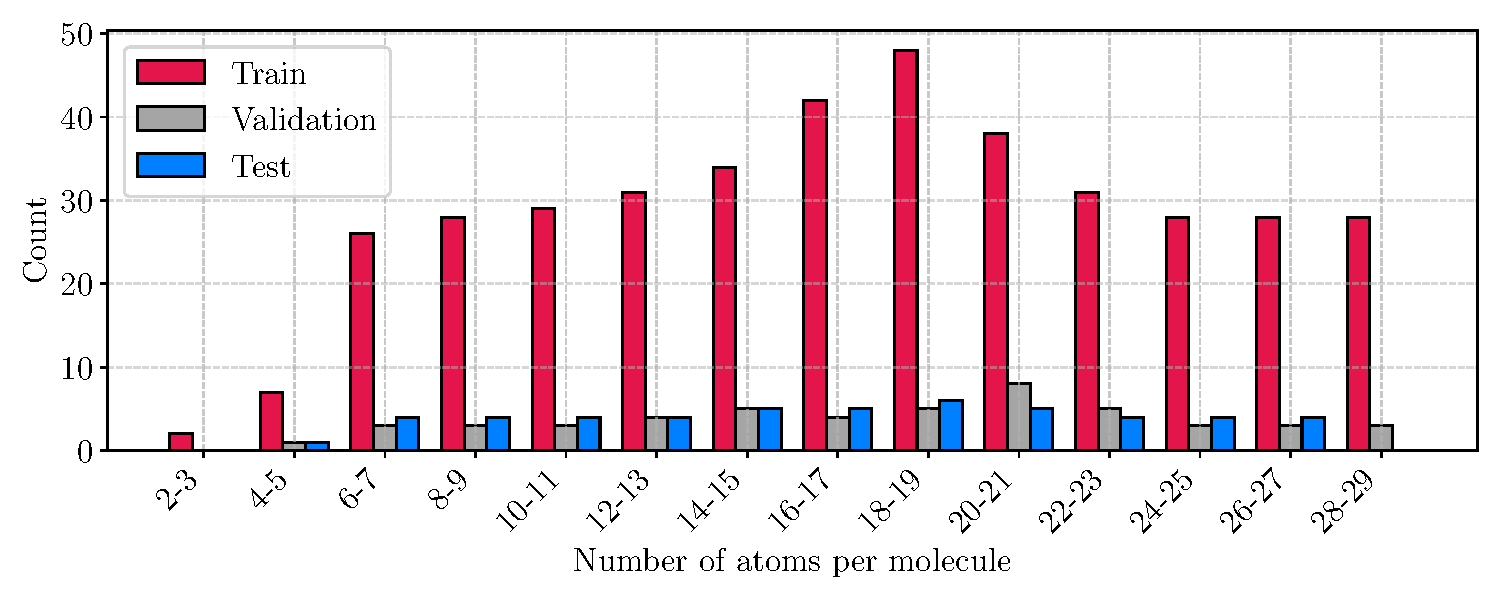
\includegraphics[width=0.9\textwidth]{../fig/application/strat_sample.pdf}
    \caption[Stratified sample of QM9 dataset]{Stratified sample of QM9 dataset by number of atoms per molecule for each set.}
    \label{fig:sample_QM9}
\end{figure}
We sample 500 molecules from the QM9 set in a stratified manner and additionally ensure ample representation for various molecule sizes. Therefore, compared to the actual distribution seen in \autoref{fig:method_qm9_overview}, the representation of molecules with 6 to 13 and 24 to 29 atoms per molecule is increased. This results in the distribution for the train, validation and test sets shown in \autoref{fig:sample_QM9}. Once again, the train/validation/test split is 80/10/10 per cent. %BE spelling

Zero-shot predictions like those devised in the previous section are not possible on the full dataset due to missing encoders/decoders for \ch{N}, \ch{F} and their respective interaction blocks. Therefore, we will proceed directly to hyperparameter tuning. 
\subsection{Hyperparameter tuning}
\label{sec:qm9_full_isomers_hyp_tuning}
Network hyperparameter tuning was carried out in the same manner as above, except that the maximum number of training epochs was increased to 50 to accommodate the more diverse dataset. \autoref{tab:qm9_full_further_runs} shows the results for the ten best performing models.
\begin{table}[H]
    \centering
    \caption[GNN on full QM9 dataset sample with full matrix loss]{GNN on full QM9 dataset sample using full matrix loss and a maximum of 50 epochs to train. Metrics on test set and corresponding hyperparameter settings for the ten best performing networks in terms of iterations.}
    \label{tab:qm9_full_further_runs} 
    \resizebox{\textwidth}{!}{
        \begin{tabular}{l
                        S[table-format=2.1(2)]
                        S[table-format=-4(3)]
                        S[table-format=-1.3(2)]
                        S[table-format=1.3(1)]
                        S[table-format=1.4(1)]}
            \toprule
            Models                 & {Iterations / 1} & {$|\Delta E_\text{DFT}|$ / $\unit{\hartree}$}  & {$|\delta E_\text{DFT}|$ / 1} & {DIIS error / $\unit{\hartree}$} & {RMSE / 1} \\
            \midrule %Data from server run!
            $\text{GNN}^{\text{Full}}_\text{f. 0}$ & 12(2)     & 1.2(5.5) & 0.001(0.003)  & 0.034(0.011) & 0.009(0.003) \\ 
            $\text{GNN}^{\text{Full}}_\text{f. 1}$ & \B 12.0(17)    & 0.9(1.7) & 0.001(0.0011)  & 0.034(0.013) & \B 0.009(2) \\
            $\text{GNN}^{\text{Full}}_\text{f. 2}$ & 12.0(1.8) & 1.3(4.2) & 0.001(0.002)  & 0.035(0.011) & 0.009(0.003) \\
            $\text{GNN}^{\text{Full}}_\text{f. 3}$ & 12.0(1.9) & 1.6(2.7) & 0.0010(0.0017)  & 0.034(0.013) & 0.009(0.003) \\
            $\text{GNN}^{\text{Full}}_\text{f. 4}$ & 12.0(1.7) & 0.2(2.1) & 0.0002(0.0017)  & 0.044(0.048) & 0.009(0.003) \\
            $\text{GNN}^{\text{Full}}_\text{f. 5}$ & 12.0(1.8) & 0.3(2.7) & 0.000(0.002)  & \B 0.033(13) & 0.009(0.003) \\
            $\text{GNN}^{\text{Full}}_\text{f. 6}$ & 12(2)     & 0.3(1.9) & 0.0002(13)  & \B 0.033(13) & 0.009(0.003) \\
            $\text{GNN}^{\text{Full}}_\text{f. 7}$ & 12.1(1.6) & 0.7(2.5) & 0.0007(0.0019)  & 0.038(0.018) & 0.009(0.003) \\
            $\text{GNN}^{\text{Full}}_\text{f. 8}$ & 12(2)     & \B 0.1(1.9) & \B 0.0000(13)  & 0.035(0.012) & 0.009(0.003) \\
            $\text{GNN}^{\text{Full}}_\text{f. 9}$ & 12.1(1.8) & 1.3(2.3) & 0.0008(0.0013)  & 0.036(0.014) & 0.009(0.002) \\
            \bottomrule
        \end{tabular}
    }
   \resizebox{\textwidth}{!}{
    \begin{tabular}{lrrrrrrrrrr}
        \toprule
        Parameters & $\text{GNN}^{\text{Full}}_\text{f. 0}$ & $\text{GNN}^{\text{Full}}_\text{f. 1}$ & $\text{GNN}^{\text{Full}}_\text{f. 2}$ & $\text{GNN}^{\text{Full}}_\text{f. 3}$ & $\text{GNN}^{\text{Full}}_\text{f. 4}$ & $\text{GNN}^{\text{Full}}_\text{f. 5}$ & $\text{GNN}^{\text{Full}}_\text{f. 6}$ & $\text{GNN}^{\text{Full}}_\text{f. 7}$ & $\text{GNN}^{\text{Full}}_\text{f. 8}$ & $\text{GNN}^{\text{Full}}_\text{f. 9}$ \\
        \midrule
        Hidden dimension & 128 & 256 & 256 & 256 & 512 & 128 & 512 & 512 & 512 & 128 \\
        Batch size & 8 & 8 & 8 & 8 & 8 & 8 & 8 & 16 & 8 & 8 \\
        Data aug. factor & 4.00 & 1.00 & 1.00 & 1.00 & 1.00 & 2.00 & 4.00 & 3.00 & 1.00 & 2.00 \\
        Edge threshold & 3.40 & 2.58 & 3.98 & 3.21 & 2.85 & 3.29 & 3.27 & 2.72 & 3.44 & 2.30 \\
        Message passing steps & 4 & 5 & 3 & 2 & 4 & 2 & 3 & 3 & 2 & 4 \\
        Message Net dropout & 0.09 & 0.16 & 0.25 & 0.21 & 0.04 & 0.11 & 0.25 & 0.04 & 0.18 & 0.19 \\
        Message Net layers & 3 & 3 & 3 & 3 & 3 & 4 & 3 & 2 & 3 & 2 \\
        Learn rate & 6.90e-04 & 9.31e-04 & 1.61e-03 & 2.75e-04 & 8.03e-04 & 1.51e-04 & 1.26e-04 & 5.85e-04 & 1.09e-03 & 6.50e-04 \\
        Weight decay & 7.15e-05 & 5.46e-05 & 3.58e-05 & 4.69e-05 & 3.99e-04 & 6.06e-04 & 2.56e-04 & 1.45e-04 & 1.84e-05 & 1.74e-05 \\
        \bottomrule
    \end{tabular}
    }
\end{table}
Both the mean iteration count and its variability increased by about one cycle compared to the best-performing isomer models. Further analysis of iteration performance by molecule size revealed no clear correlation between atom count and the number of iterations to converge.
\subsection{Evaluation \& Conclusion}
\label{sec:qm9_full_isomers_conclusion}
Using our stratified QM9 sample, we show that our GNN implementation trained on just 400 molecules achieves lower SCF iteration counts than every other guessing scheme except \texttt{minao}. The greater chemical diversity in this subset leads to a uniformly higher standard deviation in cycle counts across all methods. \autoref{tab:qm9_full_test_overview} compares our top-performing GNN against the established guessing schemes.

Another notable finding emerges when contrasting the full dataset results for $\overline{P}$ with those from the isomer only runs. While the average number of iterations remained essentially unchanged, with only their spread increasing for the more diverse dataset, the DIIS error in the full dataset differs substantially from that in the isomer-only case. Furthermore, \texttt{minao} has the second highest DIIS error while simultaneously offering the fastest converging guess. Crucially, it once again underscores that DIIS error and iteration count are largely uncorrelated. 
\begin{table}[H]
    \centering
    \caption[Models compared to \textsc{PySCF} and $\overline{P}$ schemes - full QM9 dataset]{Comparison of GNN model with calculations employing \textsc{PySCF} and $\overline{P}$ guessing schemes on the full QM9 dataset. Here, $\overline{P}$ is computed blockwise across all molecules by averaging over each \ch{C}-\ch{C}, \ch{O}-\ch{H}, etc. block.
}
    \label{tab:qm9_full_test_overview}
    \resizebox{\textwidth}{!}{
        \begin{tabular}{l
                        S[table-format=2.1(1.1)]
                        S[table-format=-3.4(3)]
                        S[table-format=-1.6(1.1)]
                        S[table-format=1.3(1.1)]
                        S[table-format=1.4(1.1)]}
                        \toprule
                        Guessing schemes                 & {Iterations / 1} & {$|\Delta E_\text{DFT}|$ / $\unit{\hartree}$}  & {$|\delta E_\text{DFT}|$ / 1} & {DIIS error / $\unit{\hartree}$} & {RMSE / 1} \\
                        \midrule
                        $\text{GNN}^{\text{Full}}_\text{f. 1}$ & 12.0(17)& \B 0.9(1.7) & \B 0.001(11)  & 0.034(0.013) & \B 0.009(2) \\
                        $\overline{P}$                & 17(3)            & 40(19)     &  0.024(10)   & 0.042(6)  & 0.014(3)  \\
                        \texttt{1-e}                  & 19(3)            & 200(80)    &  0.13(4)     & 0.122(15) & 0.16(12)  \\
                        \texttt{vsap}                 & 14(2)            & 4.3(19)    &  0.0027(9)   & \B 0.024(3)  & 0.0106(14)\\
                        \texttt{atom}                 & 16(2)            & 10(5)      &  0.006(3)    & 0.039(7)  & 0.015(2)  \\
                        \texttt{minao}                & \B 11.1(11)& \B 2.4(8) & \B 0.0016(5)& 0.081(12) & 0.017(3)  \\
                        \bottomrule
                    \end{tabular}
    }
\end{table}